% ==== Colores estilo TAB10 ====
\definecolor{accblue}{RGB}{31,119,180}    % TEκ_α (azul)
\definecolor{accorange}{RGB}{255,127,14}  % TEKTE-Net Gaussian (naranja)
\definecolor{accgreen}{RGB}{44,160,44}    % TEKTE-Net RQ (verde)

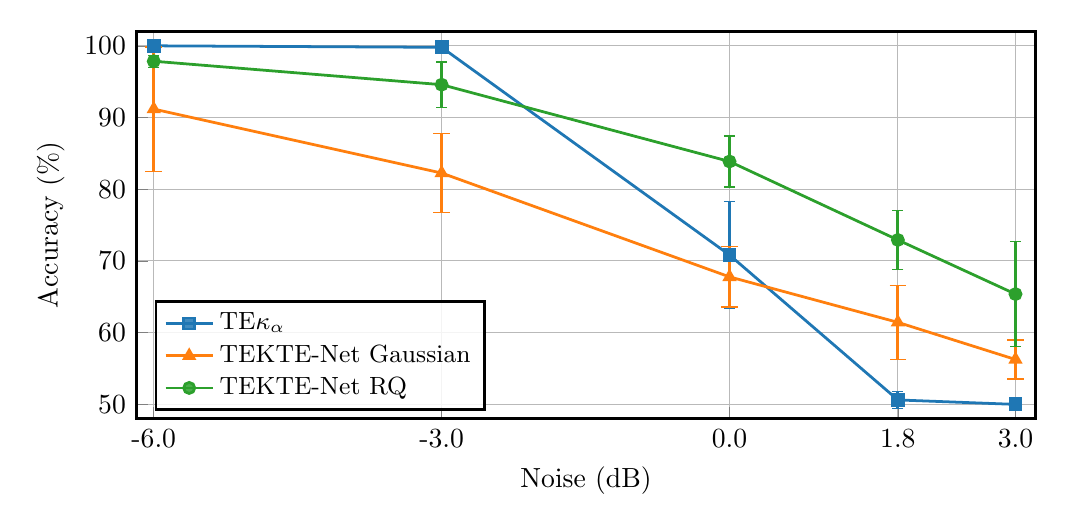
\begin{tikzpicture}
\begin{axis}[
  width=13cm,
  height=6.5cm,
  xlabel={Noise (dB)},
  ylabel={Accuracy (\%)},
  xmin=-6.2, xmax=3.2,
  xtick={-6.02,-3.01,0,1.76,2.99},
  xticklabels={-6.0,-3.0,0.0,1.8,3.0},
  ymin=48, ymax=102,
  ytick={50,60,70,80,90,100},
  axis on top=false,
  tick align=inside,
  xtick pos=bottom,
  ytick pos=left,
  grid=both,
  major grid style={draw=gray!55, line width=0.35pt},
  minor grid style={draw=gray!35, line width=0.25pt},
  xminorgrids=true,
  yminorgrids=true,
  line width=1pt,
  mark size=2pt,
  xticklabel style={align=center},
  enlarge x limits=false,
  enlarge y limits=false,
  % --- Headroom arriba para que la leyenda NO tape las curvas ---
  % enlarge y limits={upper, value=0.10},
  legend cell align=left,
  legend style={
    at={(axis description cs:0.02,0.02)},
    anchor=south west,
    draw=black,
    fill=white,
    fill opacity=0.85, text opacity=1,
    font=\small,
    nodes={align=left}
},
]
% ===== TE kappa_alpha =====
\addplot+[
  color=accblue,
  mark=square*,
  mark options={solid, fill=accblue, draw=accblue},
  error bars/.cd,
    y dir=both, y explicit,
    error bar style={line width=1pt},
    error mark=|,
    error mark options={mark size=2pt}
] coordinates {
  (-6.02, 100.00) +- (0, 0.00)
  (-3.01,  99.79) +- (0, 0.36)
  ( 0.00,  70.83) +- (0, 7.40)
  ( 1.76,  50.62) +- (0, 1.23)
  ( 2.99,  50.00) +- (0, 0.00)
};
\addlegendentry{TE$\kappa_\alpha$}
% ===== Gaussian =====
\addplot+[
  color=accorange,
  mark=triangle*,
  mark options={solid, draw=accorange, fill=accorange},
  error bars/.cd,
    y dir=both, y explicit,
    error bar style={line width=1pt},
    error mark=|,
    error mark options={mark size=3pt}
] coordinates {
  (-6.02, 91.18) +- (0, 8.65)
  (-3.01, 82.26) +- (0, 5.51)
  ( 0.00, 67.78) +- (0, 4.20)
  ( 1.76, 61.44) +- (0, 5.19)
  ( 2.99, 56.26) +- (0, 2.72)
};
\addlegendentry{TEKTE-Net Gaussian}
% ===== RQ =====
\addplot+[
  color=accgreen,
  mark=*,
  mark options={solid, fill=accgreen, draw=accgreen},
  error bars/.cd,
    y dir=both, y explicit,
    error bar style={line width=1pt},
    error mark=|,
    error mark options={mark size=2pt}
] coordinates {
  (-6.02, 97.85) +- (0, 0.82)
  (-3.01, 94.58) +- (0, 3.17)
  ( 0.00, 83.87) +- (0, 3.56)
  ( 1.76, 72.93) +- (0, 4.16)
  ( 2.99, 65.38) +- (0, 7.34)
};
\addlegendentry{TEKTE-Net RQ}
\end{axis}
\end{tikzpicture}
